\documentclass{beamer}\usepackage[]{graphicx}\usepackage[]{xcolor}
% maxwidth is the original width if it is less than linewidth
% otherwise use linewidth (to make sure the graphics do not exceed the margin)
\makeatletter
\def\maxwidth{ %
  \ifdim\Gin@nat@width>\linewidth
    \linewidth
  \else
    \Gin@nat@width
  \fi
}
\makeatother

\definecolor{fgcolor}{rgb}{0.345, 0.345, 0.345}
\newcommand{\hlnum}[1]{\textcolor[rgb]{0.686,0.059,0.569}{#1}}%
\newcommand{\hlstr}[1]{\textcolor[rgb]{0.192,0.494,0.8}{#1}}%
\newcommand{\hlcom}[1]{\textcolor[rgb]{0.678,0.584,0.686}{\textit{#1}}}%
\newcommand{\hlopt}[1]{\textcolor[rgb]{0,0,0}{#1}}%
\newcommand{\hlstd}[1]{\textcolor[rgb]{0.345,0.345,0.345}{#1}}%
\newcommand{\hlkwa}[1]{\textcolor[rgb]{0.161,0.373,0.58}{\textbf{#1}}}%
\newcommand{\hlkwb}[1]{\textcolor[rgb]{0.69,0.353,0.396}{#1}}%
\newcommand{\hlkwc}[1]{\textcolor[rgb]{0.333,0.667,0.333}{#1}}%
\newcommand{\hlkwd}[1]{\textcolor[rgb]{0.737,0.353,0.396}{\textbf{#1}}}%
\let\hlipl\hlkwb

\usepackage{framed}
\makeatletter
\newenvironment{kframe}{%
 \def\at@end@of@kframe{}%
 \ifinner\ifhmode%
  \def\at@end@of@kframe{\end{minipage}}%
  \begin{minipage}{\columnwidth}%
 \fi\fi%
 \def\FrameCommand##1{\hskip\@totalleftmargin \hskip-\fboxsep
 \colorbox{shadecolor}{##1}\hskip-\fboxsep
     % There is no \\@totalrightmargin, so:
     \hskip-\linewidth \hskip-\@totalleftmargin \hskip\columnwidth}%
 \MakeFramed {\advance\hsize-\width
   \@totalleftmargin\z@ \linewidth\hsize
   \@setminipage}}%
 {\par\unskip\endMakeFramed%
 \at@end@of@kframe}
\makeatother

\definecolor{shadecolor}{rgb}{.97, .97, .97}
\definecolor{messagecolor}{rgb}{0, 0, 0}
\definecolor{warningcolor}{rgb}{1, 0, 1}
\definecolor{errorcolor}{rgb}{1, 0, 0}
\newenvironment{knitrout}{}{} % an empty environment to be redefined in TeX

\usepackage{alltt}
\usepackage{graphicx}
\usepackage{graphicx}
\usepackage{verbatim}
\usepackage{etoolbox}
\usepackage{everysel}
% \usepackage{enumitem}

%% This package allows text highlighting
\usepackage{soul}

%% This sets the theme of the presentation which controls
%% the formatting of the slides
\usetheme{Boadilla}

%% Turn off the navigation symbols
\setbeamertemplate{navigation symbols}{} 

%% Change the default itemize [ball]s to [circle]s
\setbeamertemplate{itemize items}[circle]

%% Change the default enumerate [ball]s to plain text
\setbeamertemplate{enumerate items}[default]

%% Load the enumitem package and ensure it works nicely with beamer
% \setitemize{label=\usebeamerfont*{itemize item}
%   \usebeamercolor[fg]{itemize item}
%   \usebeamertemplate{itemize item}}
% \setenumerate{label=\usebeamerfont*{enumerate item}
%   \usebeamercolor[fg]{enumerate item}
%   \usebeamertemplate{enumerate item}}

%% Set the author block so STATS 201/8 appears on every
\author{STATS 201/8}

%% Clear the date block
\date{}


\setbeamercolor{title}{bg=blue!40}
\setbeamerfont{title}{size=\LARGE,series=\bfseries}

%%Sectioning commands
\setbeamercolor{section title}{bg=blue!20}
\setbeamerfont{section title}{size=\large}

\setbeamertemplate{section page}{%
    \begingroup
        \begin{beamercolorbox}[sep=10pt,center,rounded=true,shadow=true]{section title}
        \usebeamerfont{section title}Section~\thechapter.\thesection \newline \insertsection\par
        \end{beamercolorbox}
		\vfill
    \endgroup
}

\newcommand{\BeginSection}[1]{\section{#1} \frame{\sectionpage}}
%\AtBeginSection[]{%
%    \begin{frame}
%        \sectionpage
%    \end{frame}
%}


%% This makes all equations blue
\AtBeginEnvironment{equation*}{\color{blue}}
\AtBeginEnvironment{align*}{\color{blue}}
\everymath{\color{blue}}

%% This puts a 0 point space between paragraphs, means we don't need to use vspace, or list environments if 
%% we don't want to
\setlength{\parskip}{0pt}


%% Russell: removes spaces after R input/output?
\setlength{\topsep}{0.5mm}

%% David: In addition to Russel's command to remove spaces after R input/output, these commands remove the space between R input/output.
%% Stackoverflow link: https://stackoverflow.com/questions/35734525/reduce-space-between-code-chunks-and-code-output-in-rmarkdown-beamer-presentatio
%% \setlength{\OuterFrameSep}{-2pt}
\makeatletter
\preto{\@verbatim}{\topsep=-1pt \partopsep=-1pt }
\makeatother

%% Some useful colors
\definecolor{darkgreen}{rgb}{0.176,0.486,0.031}
\definecolor{redbrown}{HTML}{950605}
\definecolor{darkred}{HTML}{d80605}


%% nice little macro for changing the font of R code
\newcommand{\rcode}[1]{\protect{\color{darkgreen}\texttt{#1}}}

%% macro for bold blue italics
\newcommand{\blueBoldEmph}[1]{{\color{blue}\textbf{\emph{#1}}}}

% ~iid macro
\newcommand{\iid }{\stackrel{iid}{\sim}}

%% Macro for t-test amd P-value
\newcommand{\ttest}{\emph{t}-test}
\newcommand{\pval}{\emph{P}-value}

%% Statistics operators 
\DeclareMathOperator{\Bias}{Bias}
\DeclareMathOperator{\Cov}{Cov}
\DeclareMathOperator*{\Cor}{Cor}
\DeclareMathOperator{\E}{E}
\DeclareMathOperator{\MSE}{MSE}
\DeclareMathOperator{\Odds}{Odds}
\DeclareMathOperator{\OR}{OR}
\DeclareMathOperator{\PMSE}{PMSE}
\DeclareMathOperator{\sd}{sd}
\DeclareMathOperator{\se}{se}
\DeclareMathOperator*{\Var}{Var}
\DeclareMathOperator{\logit}{logit}

%% Should see if can make this a mathop
\newcommand{\comb}[2]{\mbox{$\big(_{#2}^{#1}\big)$}}




\setlength{\parskip}{9pt}
\IfFileExists{upquote.sty}{\usepackage{upquote}}{}
\begin{document}
\newcommand{\thechapter}{3}


%%\chapter{Introduction to data analysis}

\title{Chapter 3: \\ Equivalence of the null linear model and the one-sample \ttest{}}
\institute{University of Auckland}

\begin{frame}
\titlepage
\end{frame}


\begin{frame}[t]
\frametitle{Learning outcomes}
In this chapter you will learn about:
\begin{center}
\vspace{16pt}
\begin{minipage}{0.8\textwidth}
  \begin{itemize}
  \item The equivalence of fitting the null model and doing a one-sample \ttest{}.
  \item The paired \ttest{}
  \item Relevant \rcode{R}-code.
  \end{itemize}
\end{minipage}
\end{center}
\end{frame}



%%%%%%%%%%%%%%%%%%%%%%%%%%%%%%%%%%%%%%%%%%%%%%%%%%%%%%%%%%%%%%%%%%%%%%%%%%%%%%%%%%%%%%%%%%%
\BeginSection{Revisiting the null model}
%%%%%%%%%%%%%%%%%%%%%%%%%%%%%%%%%%%%%%%%%%%%%%%%%%%%%%%%%%%%%%%%%%%%%%%%%%%%%%%%%%%%%%%%%%%



\begin{frame}[fragile]
\frametitle{Null vs simple linear regression fits}

We have already encountered an example of the null model in Chapter 1.

We saw that we could explain approximately 59\% of the variation of $Exam$ by fitting a straight line model using $Test$. 
We calculated  this by comparing the sums-of-squares of the residuals for the simple linear model to the sums-of-squares of the residuals of the null model and noticed it had decreased by 59\% (ie., $R^2=$ 0.59).

In this chapter we will examine the null model in greater detail and see that it is equivalent to applying the t-distribution for obtaining confidence intervals, and to the  one-sample \ttest{} of the null hypothesis that the population mean is zero.

It is also the model we need to use when we have paired comparisons  --  two repeated measures on the same subject.
\end{frame}


\begin{frame}[fragile]
\frametitle{Null vs simple linear regression fits...}
\framesubtitle{Exam vs.\ Test marks}
If $y=\rcode{Exam}$ and $x=\rcode{Test}$, then here are our fitted null (the {\color{red} red} line) and linear (the {\color{blue} blue} line) models.

% Null model: $Y=\beta_0+\varepsilon$ ({\color{red}red}) versus 
% $Y=\beta_0+\beta_1 X+\varepsilon$ ({\color{blue}blue}) where $\varepsilon\iid N(0,\sigma^2)$:



\begin{figure}
  \centering
  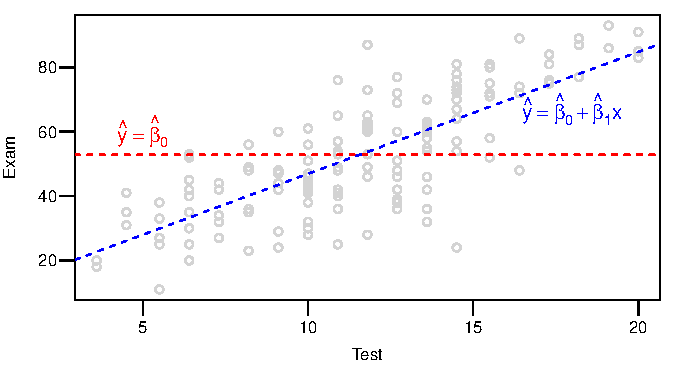
\includegraphics{figure/RC-H03-002}
\end{figure}

\end{frame}


\begin{frame}[fragile]
\frametitle{A note on the model formula}
In linear models, the intercept parameter ($\beta_0$) is fitted by default.
That is why \rcode{lm(y\textasciitilde x)} fits not just the effect of $x$, but also an intercept.
In fact, 
\rcode{lm(y\textasciitilde x)} is a shortened version of \rcode{lm(y\textasciitilde 1+x)}.
The latter form makes it explicit that the model being fitted is
\[
y =1 \times \beta_0 + x \times \beta_1  + \varepsilon,
\]
where the $\varepsilon$ are $iid$ $N(0,\sigma^2)$.
This is why the null or intercept-only model can be can be fitted using \rcode{lm(y\textasciitilde 1)} since this specifies
\[
y = 1 \times \beta_0 + \varepsilon.
\]
Since the null model is simply just specifying the mean (i.e., expected) value of $y$, it is common practive to relabel $\beta_0$ as $\mu$, in which case we have
$y = \mu + \varepsilon$. 

This can be abbreviated with the model formula $y \iid N(\mu, \sigma^{2}). $

\end{frame}



\begin{frame}
\frametitle{Inference about the expected exam mark}
{\large\bf What do we mean by ``expected exam mark''???}
(Hint: It is also called the population mean.)

Remember, the data are assumed to be a random sample from a bigger population. 

Every STATS 20x class differs a bit in the difficulty of the test and exam, for the simple reason that there are different questions every semester. The teaching staff also differ each semester......so, it would be naive to regard these data as a random sample from all STATS 20x students that we have or will ever teach.

However, it would be reasonable to assume they are from the hypothetical population of all students who could have taken STATS 20x in that particular semester.

Here we wish to see what we can say about the average, or typical, value a student in this hypothetical population will get in the exam in the absence of any other information about them. 

\end{frame}


\begin{frame}[fragile]
\frametitle{Inference about the expected exam mark\dots}
To save some typing we'll let \rcode{y} be the vector \rcode{Stats20x.df\$Exam} of exam scores.

\begin{knitrout}\scriptsize
\definecolor{shadecolor}{rgb}{0.969, 0.969, 0.969}\color{fgcolor}\begin{kframe}
\begin{alltt}
\hlstd{> }\hlstd{y}\hlkwb{=}\hlstd{Stats20x.df}\hlopt{$}\hlstd{Exam}
\hlstd{> }\hlkwd{hist}\hlstd{(y,}\hlkwc{breaks}\hlstd{=}\hlnum{20}\hlstd{,}\hlkwc{main}\hlstd{=}\hlstr{""}\hlstd{)} \hlcom{#Use main to suppress plot title}
\end{alltt}
\end{kframe}
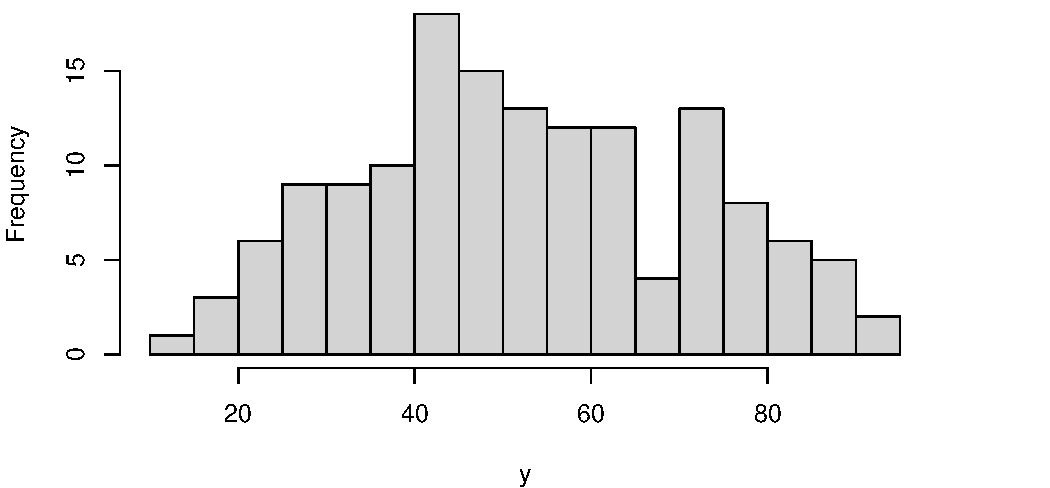
\includegraphics[width=\maxwidth]{figure/unnamed-chunk-1-1} 
\end{knitrout}
\end{frame}


\begin{frame}[fragile]
\frametitle{Inference about the expected exam mark\ldots}
\framesubtitle{Using the null model}
The histogram could be better (i.e., more normal in shape), but we'll go ahead with using the null model. We're going to be lazy\footnote{Actually, it's more like we are taking a shortcut -- the assumption checks won't tell us anything more than what we already see in the histogram of the exam marks. } and not include the assumption checks! 
\medskip

\begin{knitrout}\scriptsize
\definecolor{shadecolor}{rgb}{0.969, 0.969, 0.969}\color{fgcolor}\begin{kframe}
\begin{alltt}
\hlstd{> }\hlstd{null.fit}\hlkwb{=}\hlkwd{lm}\hlstd{(y}\hlopt{~}\hlnum{1}\hlstd{)}
\hlstd{> }\hlkwd{coef}\hlstd{(}\hlkwd{summary}\hlstd{(null.fit))} \hlcom{#Only give coefficients from summary}
\end{alltt}
\begin{verbatim}
            Estimate Std. Error  t value     Pr(>|t|)
(Intercept) 52.87671   1.545802 34.20666 2.632011e-71
\end{verbatim}
\begin{alltt}
\hlstd{> }\hlkwd{confint}\hlstd{(null.fit)}
\end{alltt}
\begin{verbatim}
              2.5 %   97.5 %
(Intercept) 49.8215 55.93193
\end{verbatim}
\end{kframe}
\end{knitrout}
\end{frame}



\begin{frame}
\frametitle{Inference about the expected exam mark\ldots}
\framesubtitle{Using the null model\ldots}
Conclusions

\begin{itemize}
\item The near zero \rcode{Pr(>|t|)} p-value totally rejects the null hypothesis that $H_0: \mu \equiv \beta_0 =0$.
\item The 95\% confidence interval for $\mu$ is 49.82 to 55.93.
\end{itemize}
\bigskip

The confidence interval is useful... but the p-value for $H_0: \mu =0$ is absolutely useless since we would never be interested in asking whether $\mu=0$.
\end{frame}



\begin{frame}
\frametitle{Inference about the expected exam mark\ldots}
\framesubtitle{A more meaningful null hypothesis}

It might be more interesting to test a hypothesis like $H_0: \mu = 60$, say, where we suppose that 60 corresponds to the target expected score when lecturers prepare STATS 20x exams.\footnote{FYI, in recent semesters the average test and exam scores have been around 70.}

Note that the above null hypothesis is $H_0: \E[Y] = 60$ and is equivalent to $H_0: \E[Y-60] = 0$.

So, if we use the response variable $y-60$ instead of $y$ then we can get a \pval{} for this $H_0$ using the \rcode{lm} function, as shown on the next slide.
\end{frame}


\begin{frame}[fragile]
\frametitle{Inference about the expected exam mark\ldots}
\framesubtitle{A more meaningful null hypothesis\ldots}

\begin{knitrout}\scriptsize
\definecolor{shadecolor}{rgb}{0.969, 0.969, 0.969}\color{fgcolor}\begin{kframe}
\begin{alltt}
\hlstd{> }\hlstd{null.fit60}\hlkwb{=}\hlkwd{lm}\hlstd{(}\hlkwd{I}\hlstd{(y}\hlopt{-}\hlnum{60}\hlstd{)}\hlopt{~}\hlnum{1}\hlstd{)}
\hlstd{> }\hlkwd{coef}\hlstd{(}\hlkwd{summary}\hlstd{(null.fit60))}
\end{alltt}
\begin{verbatim}
             Estimate Std. Error   t value     Pr(>|t|)
(Intercept) -7.123288   1.545802 -4.608151 8.828149e-06
\end{verbatim}
\end{kframe}
\end{knitrout}

Here we have used the inhibit function \rcode{I()} to prevent \rcode{lm} from mis-interpreting the model formula.
\bigskip

We see that the sample average exam score is about 4.61 standard errors below the target population exam score. The small p-value shows that this is implausible under the null hypothesis.
\bigskip

%QUESTION
{\bf Question:} In plain English, how would you state our conclusion?

\end{frame}




%%%%%%%%%%%%%%%%%%%%%%%%%%%%%%%%%%%%%%%%%%%%%%%%%%%%%%%%%%%%%%%%%%%%%%%%%%%%%%%%%%%%%%%%%%%
\BeginSection{Revisiting the $t$-test}
%%%%%%%%%%%%%%%%%%%%%%%%%%%%%%%%%%%%%%%%%%%%%%%%%%%%%%%%%%%%%%%%%%%%%%%%%%%%%%%%%%%%%%%%%%%

\begin{frame}
\frametitle{Inference about the population mean\ldots}
\framesubtitle{Using the $t$-test}
Recall from STATS 10x that we can use the $t$-distribution to make inference about
$\mu$ when  $y \iid N(\mu, \sigma^{2})$.

First, we will do it the hard way, by hand.

Then, we'll let R do it for us.
\end{frame}



\begin{frame}[fragile]
\frametitle{Inference about the population mean\ldots}
\framesubtitle{Using the $t$-test\ldots}
It can be shown (in STATS 310) that 
\[
T = \frac{\overline{y}-\mu}{\frac{s}{\sqrt{n}}} \sim t_{n-1},
\]
where $\overline{y}$ and $s$ are the sample mean and sample standard deviation we calculate from our sample.\footnote{Recall that this is interpretted as being the distribution of $T$ when the experiment is repeated. That is, if other random samples are taken from the population.}

We can use this result to do hypothesis tests and get confidence intervals about the quantity of interest, $\mu$ (the population mean exam mark).\footnote{Recall that $T$ is $t_{n-1}$-distributed rather than normal as we have additional variability from using $s^2$ to estimate $\sigma^2$.} 
\end{frame}



\begin{frame}[fragile]
\frametitle{Inference about the population mean\ldots}
\framesubtitle{Calculating the $t$-value} 

In 10x you were taught how to calculate a 95\%  CI for $\mu$ from your sample of $n$ observations having
sample mean $\bar{y}$ and sample standard deviation $s$:
\[
\bar{y}\pm t_{n-1}^{(0.975)}\frac{s}{\sqrt{n}}
\]
where $t_{n-1}^{(0.975)}$ is the $t$-multiplier. For a  95\% CI this multiplier is pretty close to 2 provided that $n>30$.
\footnote{ In this example, $t_{n-1}^{(0.975)}=t_{145}^{(0.975)}=1.97646\approx 2.$}
\end{frame}


\begin{frame}[fragile]
\frametitle{Inference about the population mean\ldots}
\framesubtitle{Calculating the $t$-value\ldots}
Let us calculate the t-statistic for the null hypothesis that $\mu=60$.
This is
\[
T = \frac{\bar{y}-60}{\frac{s}{\sqrt{n}}} .
\]

\begin{knitrout}\scriptsize
\definecolor{shadecolor}{rgb}{0.969, 0.969, 0.969}\color{fgcolor}\begin{kframe}
\begin{alltt}
\hlstd{> }\hlstd{n}\hlkwb{=}\hlkwd{length}\hlstd{(y)} \hlcom{#146 students}
\hlstd{> }\hlstd{tstat}\hlkwb{=}\hlstd{(}\hlkwd{mean}\hlstd{(y)}\hlopt{-}\hlnum{60}\hlstd{)}\hlopt{/}\hlstd{(}\hlkwd{sd}\hlstd{(y)}\hlopt{/}\hlkwd{sqrt}\hlstd{(n))}
\hlstd{> }\hlstd{tstat}
\end{alltt}
\begin{verbatim}
[1] -4.608151
\end{verbatim}
\end{kframe}
\end{knitrout}

How does this $t$-value compare to the one from \rcode{ coef(summary(null.fit60))} that we saw a few pages earlier?
\end{frame}


\begin{frame}[fragile]
\frametitle{Inference about the population mean\ldots}
\framesubtitle{Calculating the confidence interval} 
Let us now manually compute a 95\% CI based on the \textit{t}-distribution:
\begin{knitrout}\scriptsize
\definecolor{shadecolor}{rgb}{0.969, 0.969, 0.969}\color{fgcolor}\begin{kframe}
\begin{alltt}
\hlstd{> }\hlcom{## t-multiplier}
\hlstd{> }\hlstd{tmult} \hlkwb{=} \hlkwd{qt}\hlstd{(}\hlnum{1}\hlopt{-}\hlnum{.05}\hlopt{/}\hlnum{2}\hlstd{,} \hlkwc{df}\hlstd{=n}\hlopt{-}\hlnum{1}\hlstd{)}
\hlstd{> }\hlcom{## We want the upper 97.5% (or 1-.05/2) bound of the CI}
\hlstd{> }\hlcom{## NOTE: mean = sample mean; sd = standard deviation; sqrt = square root}
\hlstd{> }\hlkwd{mean}\hlstd{(y)} \hlopt{-} \hlstd{tmult}\hlopt{*}\hlkwd{sd}\hlstd{(y)}\hlopt{/}\hlkwd{sqrt}\hlstd{(n)}
\end{alltt}
\begin{verbatim}
[1] 49.8215
\end{verbatim}
\begin{alltt}
\hlstd{> }\hlcom{## Upper bound of CI}
\hlstd{> }\hlkwd{mean}\hlstd{(y)} \hlopt{+} \hlstd{tmult}\hlopt{*}\hlkwd{sd}\hlstd{(y)}\hlopt{/}\hlkwd{sqrt}\hlstd{(n)}
\end{alltt}
\begin{verbatim}
[1] 55.93193
\end{verbatim}
\begin{alltt}
\hlstd{> }\hlcom{## Or if we want both the lower and upper bounds of the CI in one statement}
\hlstd{> }\hlkwd{mean}\hlstd{(y)} \hlopt{+} \hlkwd{c}\hlstd{(}\hlopt{-}\hlnum{1}\hlstd{,}\hlnum{1}\hlstd{)}\hlopt{*}\hlstd{tmult}\hlopt{*}\hlkwd{sd}\hlstd{(y)}\hlopt{/}\hlkwd{sqrt}\hlstd{(n)}
\end{alltt}
\begin{verbatim}
[1] 49.82150 55.93193
\end{verbatim}
\end{kframe}
\end{knitrout}
How does this CI compare to the one from \rcode{confint(null.fit)}?
\end{frame}



\begin{frame}[fragile]
\frametitle{Inference about the population mean\ldots}
\framesubtitle{The \rcode{t.test} function in R} 
Of course, R has a convenient function to do the \ttest{} calculations for us.

To test $H_0: \mu=60$, we include \rcode{mu=60} in the call of \rcode{t.test}

\begin{knitrout}\scriptsize
\definecolor{shadecolor}{rgb}{0.969, 0.969, 0.969}\color{fgcolor}\begin{kframe}
\begin{alltt}
\hlstd{> }\hlkwd{t.test}\hlstd{(y,}\hlkwc{mu}\hlstd{=}\hlnum{60}\hlstd{)}
\end{alltt}
\begin{verbatim}

	One Sample t-test

data:  y
t = -4.6082, df = 145, p-value = 8.828e-06
alternative hypothesis: true mean is not equal to 60
95 percent confidence interval:
 49.82150 55.93193
sample estimates:
mean of x 
 52.87671 
\end{verbatim}
\end{kframe}
\end{knitrout}
\end{frame}



\begin{frame}[fragile]
\frametitle{Inference about the population mean\ldots}
\framesubtitle{The null model versus the \ttest{}} 

We've seen that we get the same results from using the null model as we do from using the \ttest{}. This is because they are both based on the same statistical theory.
\medskip

The null model is a special case (in fact, it is the simplest case) of a linear model.\footnote{If you have done some maths courses, you might recall that a linear model is one that has constant derivative with respect to its coefficients} 

\medskip
For completeness we will also look at using the bootstrap, 
which you saw in STATS 10x --
recall that the bootstrap samples {\bf with replacement} from the data.
\end{frame}

%%%%%%%%%%%%%%%%%%%%%%%%%%%%%%%%%%%%%%%%%%%%%%%%%%%%%%%%%%%%%%%%%%%%%%%%%%%%%%%%%%%%%%%%%%%
\BeginSection{Inference about $\mu$ using the bootstrap \\ (Non examinable)}
%%%%%%%%%%%%%%%%%%%%%%%%%%%%%%%%%%%%%%%%%%%%%%%%%%%%%%%%%%%%%%%%%%%%%%%%%%%%%%%%%%%%%%%%%%%


\begin{frame}[fragile]
\frametitle{Inference about the population mean\ldots}
\framesubtitle{Bootstrapping}

\begin{knitrout}\scriptsize
\definecolor{shadecolor}{rgb}{0.969, 0.969, 0.969}\color{fgcolor}\begin{kframe}
\begin{alltt}
\hlstd{> }\hlcom{## Resampling the exam marks, N times with replacement:}
\hlstd{> }\hlstd{N}\hlkwb{=}\hlnum{10000} \hlcom{# The number of bootstrap resamples we want}
\hlstd{> }\hlcom{# The new sample means are stored in ybar}
\hlstd{> }\hlstd{ybar}\hlkwb{=}\hlkwd{rep}\hlstd{(}\hlnum{NA}\hlstd{,N)} \hlcom{## A vector of length N to store our resampled means}
\hlstd{> }
\hlstd{> }\hlcom{## A loop - allows us to do something N (10,000) times}
\hlstd{> }\hlkwa{for} \hlstd{(i} \hlkwa{in} \hlnum{1}\hlopt{:}\hlstd{N)\{}
\hlstd{+ }  \hlcom{## Take the average of this sample (below) from a sample of size n = 146 from y - with replacement}
\hlstd{+ }  \hlstd{ybar[i]}\hlkwb{=}\hlkwd{mean}\hlstd{(} \hlkwd{sample}\hlstd{(y,n,} \hlkwc{replace}\hlstd{=T) )}
\hlstd{+ }\hlstd{\}}
\hlstd{> }\hlkwd{mean}\hlstd{(ybar)}
\end{alltt}
\begin{verbatim}
[1] 52.84468
\end{verbatim}
\end{kframe}
\end{knitrout}
\bigskip

Here is a simpler way of doing the bootstrap, but it requires the \rcode{bootstrap} package to be installed:
\begin{knitrout}\scriptsize
\definecolor{shadecolor}{rgb}{0.969, 0.969, 0.969}\color{fgcolor}\begin{kframe}
\begin{alltt}
\hlstd{> }\hlkwd{library}\hlstd{(bootstrap)}
\hlstd{> }\hlstd{ybar} \hlkwb{=} \hlkwd{bootstrap}\hlstd{(y,} \hlnum{10000}\hlstd{, mean)}\hlopt{$}\hlstd{thetastar}
\end{alltt}
\end{kframe}
\end{knitrout}

\end{frame}


\begin{frame}[fragile]
\frametitle{Inference about the population mean\ldots}
\framesubtitle{Bootstrapping \ldots}
\vspace{3mm}
\begin{knitrout}\scriptsize
\definecolor{shadecolor}{rgb}{0.969, 0.969, 0.969}\color{fgcolor}\begin{kframe}
\begin{alltt}
\hlstd{> }\hlcom{## Histogram of these 10,000 bootstrap means}
\hlstd{> }\hlkwd{hist}\hlstd{(ybar,}\hlkwc{xlab}\hlstd{=}\hlstr{"Bootstrapped sample means"}\hlstd{)}
\end{alltt}
\end{kframe}
\end{knitrout}



\begin{figure}
  \centering
  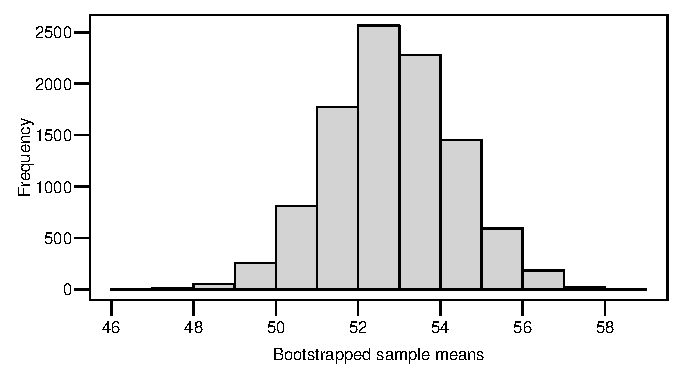
\includegraphics{figure/RC-H03-008}
\end{figure}

\end{frame}

\begin{frame}[fragile]
\frametitle{Inference about the population mean\ldots}
\framesubtitle{Bootstrapping \ldots} 

This looks very 'Normal'. 

\textbf{Note:} the mean value of \rcode{ybar}, 52.84, is about the same as that of the original sample (52.88),  
but the values have less scatter. They have lower quartile of 51.8 (in the original sample it was 40),
and upper quartile 53.9 (versus 68.5).

A 95\% bootstrap confidence interval for the expected exam mark is given by the following code:
\begin{knitrout}\scriptsize
\definecolor{shadecolor}{rgb}{0.969, 0.969, 0.969}\color{fgcolor}\begin{kframe}
\begin{alltt}
\hlstd{> }\hlcom{## 2.5% in the lower tail and 2.5% in the upper tail}
\hlstd{> }\hlkwd{quantile}\hlstd{(ybar,} \hlkwd{c}\hlstd{(}\hlnum{.025}\hlstd{,} \hlnum{.975}\hlstd{))}
\end{alltt}
\begin{verbatim}
    2.5%    97.5% 
49.86301 55.85616 
\end{verbatim}
\end{kframe}
\end{knitrout}

We say: We are 95\% confident that the expected exam mark 
is somewhere between 49.9 to 55.9 marks.\footnote{The magic of the bootstrap is that these
quantiles of the bootstrapped means give a CI for the population mean -- see STATS 730 for proof of this.} 
\end{frame}


\begin{frame}[fragile]
\frametitle{Inference about the population mean\ldots}
\framesubtitle{Bootstrapping\ldots} 
Here is the distribution of sample means we bootstrapped, with a density plot (in {\color{blue}blue} -- which can be though of as a `fine-grain' histogram), along with the underlying theoretical Normal based-distribution (in {\color{red}red}):


\begin{figure}
  \centering
  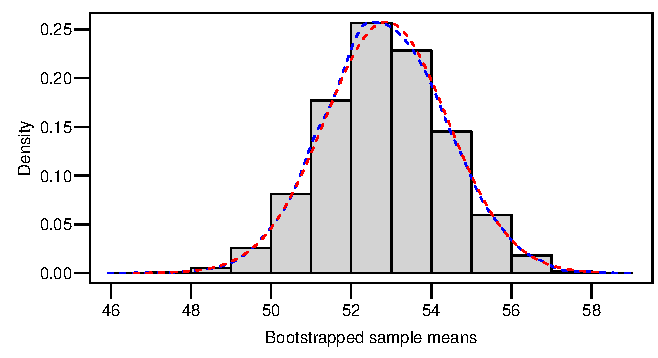
\includegraphics{figure/RC-H03-010}
\end{figure}

\end{frame}


\begin{frame}[fragile]
\frametitle{Inference about the population mean\ldots}
\framesubtitle{Bootstrapping and the \textit{t}-distribution}  
So what is going on here? 
Provided we have a large enough sample, 
we know that the distribution of all possible sample means we could have obtained from repeating the experiment is distributed approximately normally\footnote{There are some other necessary conditions 
but this holds for most populations.} 
and hence, these sample means can be described well with a normal distribution.

\medskip

This is known as the \textbf{Central limit effect} or \textbf{theorem}, referred henceforth as the \textbf{CLT}. Both the bootstrap and \textit{t}-distribution follow the CLT.
\end{frame}

\begin{frame}[fragile]
\frametitle{Inference about the population mean\ldots}
\framesubtitle{Bootstrapping and the \textit{t}-distribution\ldots}  
Let us compare the bootstrap CI to the \textit{t}-distribution CI:
\begin{knitrout}\scriptsize
\definecolor{shadecolor}{rgb}{0.969, 0.969, 0.969}\color{fgcolor}\begin{kframe}
\begin{alltt}
\hlstd{> }\hlcom{## Bootstrap:}
\hlstd{> }\hlkwd{quantile}\hlstd{(ybar,} \hlkwd{c}\hlstd{(}\hlnum{.025}\hlstd{,} \hlnum{.975}\hlstd{))}
\end{alltt}
\begin{verbatim}
    2.5%    97.5% 
49.86301 55.85616 
\end{verbatim}
\begin{alltt}
\hlstd{> }\hlcom{## t-distribution:}
\hlstd{> }\hlkwd{mean}\hlstd{(y)} \hlopt{+} \hlkwd{c}\hlstd{(}\hlopt{-}\hlnum{1}\hlstd{,}\hlnum{1}\hlstd{)}\hlopt{*}\hlstd{tmult}\hlopt{*}\hlkwd{sd}\hlstd{(y)}\hlopt{/}\hlkwd{sqrt}\hlstd{(n)}
\end{alltt}
\begin{verbatim}
[1] 49.82150 55.93193
\end{verbatim}
\end{kframe}
\end{knitrout}

Very similar.

\textbf{Note:} From now on we will not do any more bootstrapping as it does not generalize easily to more complex models. 

\end{frame}


%%%%%%%%%%%%%%%%%%%%%%%%%%%%%%%%%%%%%%%%%%%%%%%%%%%%%%%%%%%%%%%%%%%%%%%%%%%%%%%%%%%%%%%%%%%
\BeginSection{The paired \ttest}
%%%%%%%%%%%%%%%%%%%%%%%%%%%%%%%%%%%%%%%%%%%%%%%%%%%%%%%%%%%%%%%%%%%%%%%%%%%%%%%%%%%%%%%%%%%



\begin{frame}[fragile]
\frametitle{Paired comparisons $\equiv$ one-sample \ttest{}}

Recall (from STATS 10x) that the paired t-test is just an application of the one-sample t-test
applied to differences. 
\bigskip

Here, we demonstrate this by comparing $Test$ and $Exam$ marks.

\end{frame}


\begin{frame}[fragile]
\frametitle{Comparing $Test$ and $Exam$ marks}
Suppose we want to know if the midterm test marks and exam marks have the same expected value.
Note that the test and exam scores are not independent (why?).

The data are paired since we have a test score and exam score from each student\footnote{
Two measurements on the same student constitutes a paired measure
and this is an example of a repeated (twice) measures study.}.

For a meaningful comparison, We will need to make them have the same scale, 
so we multiply the test mark by 5 so that it is also out of 100. 
This can be done very easily with the following \rcode{R} code:

\begin{knitrout}\scriptsize
\definecolor{shadecolor}{rgb}{0.969, 0.969, 0.969}\color{fgcolor}\begin{kframe}
\begin{alltt}
\hlstd{> }\hlstd{Stats20x.df}\hlopt{$}\hlstd{Test2} \hlkwb{=} \hlnum{5} \hlopt{*} \hlstd{Stats20x.df}\hlopt{$}\hlstd{Test}
\hlstd{> }\hlcom{## Check that it worked}
\hlstd{> }\hlstd{Stats20x.df[}\hlnum{1}\hlopt{:}\hlnum{3}\hlstd{,} \hlkwd{c}\hlstd{(}\hlstr{"Exam"}\hlstd{,}\hlstr{"Test"}\hlstd{,}\hlstr{"Test2"}\hlstd{)]}
\end{alltt}
\begin{verbatim}
  Exam Test Test2
1   42  9.1  45.5
2   58 13.6  68.0
3   81 14.5  72.5
\end{verbatim}
\end{kframe}
\end{knitrout}
\end{frame}


\begin{frame}[fragile]
\frametitle{Comparing $Test$ and $Exam$ marks\ldots}

We wish to see how the exam score and scaled test score (out of 100) differ. 
We might suspect that they have the same expected value $\mu$. 

\medskip 

A student who scores high on the exam would be expected to score high on the test and vice-versa. 
So these two measurements are not independent of each other. 
However, when we look at their differences (\rcode{Diff = Test2 - Exam}) these constitute a single
measurement from each student, and moreover these differences could reasonably be assumed
to be independent of each other. 
\medskip 

In effect, we have eliminated the student effect on test and exam scores by
working with the difference between test and exam for each student.
\end{frame}

\begin{frame}[fragile]
\frametitle{Comparing $Test$ and $Exam$ marks\ldots}
\framesubtitle{Calculating the difference}

Let us name the new variable \rcode{Diff} (and check that we have done it correctly):
\begin{knitrout}\scriptsize
\definecolor{shadecolor}{rgb}{0.969, 0.969, 0.969}\color{fgcolor}\begin{kframe}
\begin{alltt}
\hlstd{> }\hlstd{Stats20x.df}\hlopt{$}\hlstd{Diff} \hlkwb{=} \hlstd{Stats20x.df}\hlopt{$}\hlstd{Test2} \hlopt{-} \hlstd{Stats20x.df}\hlopt{$}\hlstd{Exam}
\hlstd{> }\hlcom{## Check the first 5 measurements}
\hlstd{> }\hlstd{Stats20x.df[}\hlnum{1}\hlopt{:}\hlnum{5}\hlstd{,} \hlkwd{c}\hlstd{(}\hlstr{"Test2"}\hlstd{,}\hlstr{"Exam"}\hlstd{,}\hlstr{"Diff"}\hlstd{)]}
\end{alltt}
\begin{verbatim}
  Test2 Exam Diff
1  45.5   42  3.5
2  68.0   58 10.0
3  72.5   81 -8.5
4  95.5   86  9.5
5  41.0   35  6.0
\end{verbatim}
\begin{alltt}
\hlstd{> }\hlcom{## Looks good!}
\end{alltt}
\end{kframe}
\end{knitrout}
\end{frame}


\begin{frame}[fragile]
\frametitle{Comparing $Test$ and $Exam$ marks\ldots}
\framesubtitle{Null hypothesis for the expected difference}

If test and exam scores have the same expected value, then their difference must have an expected value of 0.
We will denote this $\mu_{diff}=0$. This is our null hypothesis.

\medskip

Before we do the test of $H_0: \mu_{diff}=0$ we should do some assumption checks.

We have independence sorted, and we are necessarily assuming identical distribution.
Let us produce a histogram to check normality.
\end{frame}


\begin{frame}[fragile]
\frametitle{Comparing $Test$ and $Exam$ marks\ldots}
\framesubtitle{Inspecting the differences}
\begin{knitrout}\scriptsize
\definecolor{shadecolor}{rgb}{0.969, 0.969, 0.969}\color{fgcolor}\begin{kframe}
\begin{alltt}
\hlstd{> }\hlkwd{hist}\hlstd{(Stats20x.df}\hlopt{$}\hlstd{Diff,}\hlkwc{xlab}\hlstd{=}\hlstr{"Difference between test and exam scores"}\hlstd{)}
\end{alltt}
\end{kframe}
\end{knitrout}



\begin{figure}
  \centering
  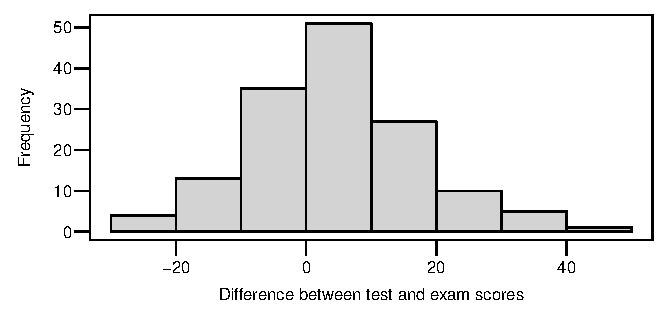
\includegraphics{figure/RC-H03-021.pdf}
\end{figure}

Looks very normalish. Let's fit a null linear model (i.e., one-sample t-test) to the differences.

\end{frame}


\begin{frame}[fragile]
\frametitle{Testing for a significant difference}

\begin{knitrout}\scriptsize
\definecolor{shadecolor}{rgb}{0.969, 0.969, 0.969}\color{fgcolor}\begin{kframe}
\begin{alltt}
\hlstd{> }\hlstd{diff.fit} \hlkwb{=} \hlkwd{lm}\hlstd{(Diff}\hlopt{~}\hlnum{1}\hlstd{,} \hlkwc{data}\hlstd{=Stats20x.df)}
\hlstd{> }\hlkwd{coef}\hlstd{(}\hlkwd{summary}\hlstd{(diff.fit))}
\end{alltt}
\begin{verbatim}
            Estimate Std. Error  t value     Pr(>|t|)
(Intercept) 4.958904   1.063718 4.661861 7.042125e-06
\end{verbatim}
\end{kframe}
\end{knitrout}

\begin{knitrout}\scriptsize
\definecolor{shadecolor}{rgb}{0.969, 0.969, 0.969}\color{fgcolor}\begin{kframe}
\begin{alltt}
\hlstd{> }\hlkwd{confint}\hlstd{(diff.fit)}
\end{alltt}
\begin{verbatim}
               2.5 %   97.5 %
(Intercept) 2.856509 7.061299
\end{verbatim}
\begin{alltt}
\hlstd{> }\hlkwd{t.test}\hlstd{(Stats20x.df}\hlopt{$}\hlstd{Diff)}
\end{alltt}
\begin{verbatim}

	One Sample t-test

data:  Stats20x.df$Diff
t = 4.6619, df = 145, p-value = 7.042e-06
alternative hypothesis: true mean is not equal to 0
95 percent confidence interval:
 2.856509 7.061299
sample estimates:
mean of x 
 4.958904 
\end{verbatim}
\end{kframe}
\end{knitrout}


\end{frame}


\begin{frame}[fragile]
\frametitle{Comparing $Test$ and $Exam$ marks\ldots}
\framesubtitle{Conclusions}
So it appears that, on average, students do worse in the exam than the term test ($\mbox{\pval{}}\approx 7\times 10^{-6}$).

We estimate this difference to be about 2.9 to 7.1 marks (out of 100).
\medskip

The exam was considerably harder than the test  --  this is something that lecturers normally try to avoid. It's not a good idea for the test to be easier than the exam, since it may lull students into a false sense of security.

\end{frame}



\begin{frame}[fragile]
\frametitle{Comparing $Test$ and $Exam$ marks\ldots}
\framesubtitle{Closing remarks}

{\bf Some history;} The \rcode{Stats20x.df} data were collected some years ago. Back then, lecturers were able to scale marks as they saw fit, and were also to choose the final grade ranges for awarding the letter grades (A+, A,...etc).

So, lecturers would often deliberately set very challenging tests and exams since they would be able to adjust grades upwards and lower the grade requirement for a letter grade. This would have been the case for the test and exam marks in \rcode{Stats20x.df}. 

Lecturers no longer have as much flexibility, and so these days test and exam (and assignment) marks must now be more representative of the final grade.

\end{frame}

%%%%%%%%%%%%%%%%%%%%%%%%%%%%%%%%%%%%%%%%%%%%%%%%%%%%%%%%%%%%%%%%%%%%%%%%%%%%%%%%%%%%%%%%%%%
\BeginSection{Relevant \rcode{R}-code}
%%%%%%%%%%%%%%%%%%%%%%%%%%%%%%%%%%%%%%%%%%%%%%%%%%%%%%%%%%%%%%%%%%%%%%%%%%%%%%%%%%%%%%%%%%%


\begin{frame}[fragile]
\frametitle{Most of the \rcode{R}-code you need for this chapter}

Fitting the model with no explanatory variables (i.e. no $x$):

\begin{knitrout}\scriptsize
\definecolor{shadecolor}{rgb}{0.969, 0.969, 0.969}\color{fgcolor}\begin{kframe}
\begin{alltt}
\hlstd{> }\hlstd{exam.fit}\hlkwb{=}\hlkwd{lm}\hlstd{(Exam}\hlopt{~}\hlnum{1}\hlstd{,} \hlkwc{data}\hlstd{=Stats20x.df)}
\hlstd{> }\hlkwd{confint}\hlstd{(exam.fit)}
\hlstd{> }\hlstd{exam.fit60}\hlkwb{=}\hlkwd{lm}\hlstd{(}\hlkwd{I}\hlstd{(Exam}\hlopt{-}\hlnum{60}\hlstd{)}\hlopt{~}\hlnum{1}\hlstd{,} \hlkwc{data}\hlstd{=Stats20x.df)}
\hlstd{> }\hlkwd{coef}\hlstd{(}\hlkwd{summary}\hlstd{(exam.fit60))}
\end{alltt}
\end{kframe}
\end{knitrout}
Equivalent output can be obtained from the t-test:

\begin{knitrout}\scriptsize
\definecolor{shadecolor}{rgb}{0.969, 0.969, 0.969}\color{fgcolor}\begin{kframe}
\begin{alltt}
\hlstd{> }\hlkwd{t.test}\hlstd{(Stats20x.df}\hlopt{$}\hlstd{Exam,}\hlkwc{mu}\hlstd{=}\hlnum{60}\hlstd{)}
\end{alltt}
\end{kframe}
\end{knitrout}

For a paired comparison we need to create the difference variable:

\begin{knitrout}\scriptsize
\definecolor{shadecolor}{rgb}{0.969, 0.969, 0.969}\color{fgcolor}\begin{kframe}
\begin{alltt}
\hlstd{> }\hlstd{Stats20x.df}\hlopt{$}\hlstd{Diff} \hlkwb{=} \hlstd{Stats20x.df}\hlopt{$}\hlstd{Test2} \hlopt{-} \hlstd{Stats20x.df}\hlopt{$}\hlstd{Exam} \hlcom{# create differences}
\end{alltt}
\end{kframe}
\end{knitrout}
\vspace{-3mm}
Then either of these will suffice:
\begin{knitrout}\scriptsize
\definecolor{shadecolor}{rgb}{0.969, 0.969, 0.969}\color{fgcolor}\begin{kframe}
\begin{alltt}
\hlstd{> }\hlcom{# confidence interval for fitted value:}
\hlstd{> }\hlstd{diff.fit}\hlkwb{=}\hlkwd{lm}\hlstd{(Diff}\hlopt{~}\hlnum{1}\hlstd{,} \hlkwc{data} \hlstd{= Stats20x.df)}
\hlstd{> }\hlkwd{coef}\hlstd{(}\hlkwd{summary}\hlstd{(diff.fit))}
\hlstd{> }\hlkwd{confint}\hlstd{(diff.fit)}
\end{alltt}
\end{kframe}
\end{knitrout}
\vspace{-3mm} or equivalently
\begin{knitrout}\scriptsize
\definecolor{shadecolor}{rgb}{0.969, 0.969, 0.969}\color{fgcolor}\begin{kframe}
\begin{alltt}
\hlstd{> }\hlkwd{t.test}\hlstd{(Stats20x.df}\hlopt{$}\hlstd{Diff)}
\end{alltt}
\end{kframe}
\end{knitrout}



\end{frame}


\end{document}

